% Options here are passed to the article class.
% Most common options: 10pt, 11pt, 12pt
\documentclass[10pt]{datasheet}

% Input encoding and typographical rules for English language
\usepackage[utf8]{inputenc}
\usepackage[english]{babel}
\usepackage[english]{isodate}

% tikz is used to draw images in this example, but you can
% also use \includegraphics{}.
\usepackage{graphicx}

% These define global texts that are used in headers and titles.
\title{EC05: Hopperspeed Encoder With Minimal Code Items}
\author{willymc}
\tags{encoders, hopperspeed}
\date{25 December 2023}
\revision{Revision 1}
\begin{document}
\maketitle

\section{Features}

\begin{itemize}
\item{Hopperspeed (9000 items/hr) encoding.}
\item{Adjustable and expandable to work with any base.}
\item{Requires only 2 items per item type per chest.}
\item{Cart yeeter based cart recycler and storage.}
\end{itemize}

\section{Applications}

\begin{itemize}
\item{Encoding items}
\end{itemize}

\section{General Description}
The EC05 encoder uses multiple hoppercarts to allow for hopperspeed item to code encoding. Unlike other hopperspeed encoders, this design only requires 2 items per item type per chest, the minimum amount possible.

\vfill\break

\begin{figure}[h]
    \centering
    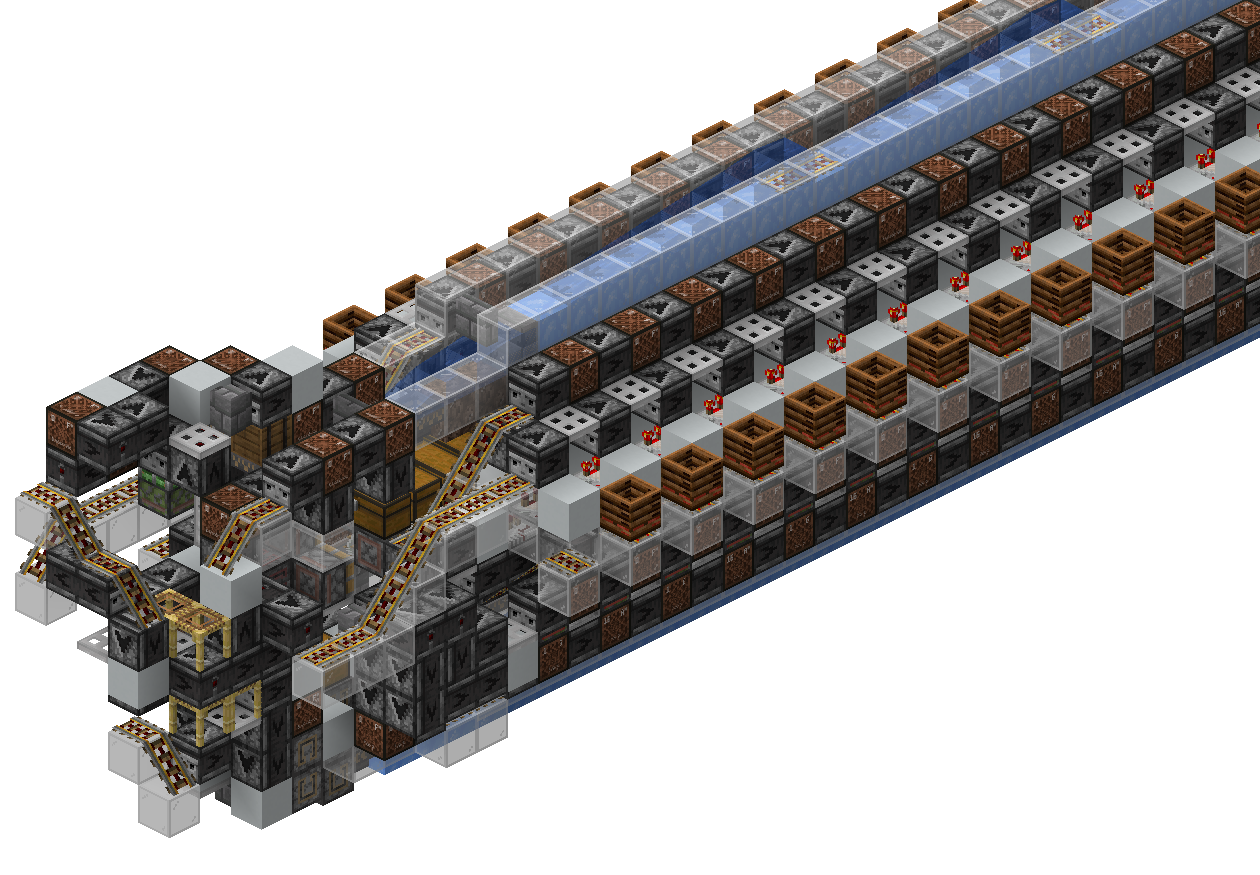
\includegraphics[width=0.48\textwidth]{pic.png}
    \caption{\centering Hopperspeed Encoder With Minimal Code Items}
\end{figure}

% For wide tables, a single column layout is better. It can be switched
% page-by-page.
\onecolumn

\section{Device Specifications}

\begin{table}[h]
    \caption{Inputs}
    \begin{tabularx}{\textwidth}{l | c | X}
        \thickhline
        \textbf{Name} & \textbf{Range} & \textbf{Description} \\
        \hline
        Box input & Box Item & Single-type box with items for encoding. \\
        \thickhline
\end{tabularx}
\end{table}

\begin{table}[h]
    \caption{Outputs}
    \begin{tabularx}{\textwidth}{l | c | X}
        \thickhline
        \textbf{Name} & \textbf{Range} & \textbf{Description} \\
        \hline
        Box output & Box Item & Outputs the inputted box timed with the code. \\
        \hline
        Code signal & Code & Outputs a redstone signal corresponding to the mapped item code. \\
        \thickhline
\end{tabularx}
\end{table}

\begin{table}[h]
    \caption{Device Specifications}
    \begin{tabularx}{\textwidth}{l | c c c | c | X}
        \thickhline
        \textbf{Parameter} & \textbf{Min.} & \textbf{Typ.} & \textbf{Max.} &
        \textbf{Unit} & \textbf{Conditions} \\
        \hline
        Throughput  & 8 & - & - & gt & Normal Usage \\
        \hline
        Active Lag & +4 & +8 & +10 & ms & At Hopperspeed. Ryzen 5 3600, 2GB RAM. MC 1.19.3 with Lithium. \\
        \hline
        MC Version & 1.19 & 1.19.3 & - & MCV & Latest version at time of writing: 1.20.4\\
        \hline
        Dimensions & & 11 x 13 x 84 & & Blocks & \\
        \thickhline
\end{tabularx}
\end{table}
\newpage
\section{Testing Data}
\begin{table}[h]
\caption{Executed Tests}
\begin{tabularx}{\textwidth}{l | X}
    \thickhline
    \textbf{Test} & \textbf{Result} \\
    \hline
    Box encoding test & Device was able to encode with box input \\
    \hline
    Throughput test & Device was able to encode at 8gt throughput with randomized input. Four different codes were set with items in consecutive chests. \\
    \thickhline
\end{tabularx}
\end{table}

\section{Download Information}
\begin{table}[h]
    \caption{Download Information}
    \begin{tabularx}{\textwidth}{l | l | l | X}
        \thickhline
        \textbf{Identifier} & \textbf{MC} & \textbf{File} & \textbf{Description} \\
        \hline
        EC05 & 1.19.3 & \href{https://github.com/Soontech-Annals/Archive/blob/364bde8dbcbc2e5337489ff435bcda9b387017e2/Archive/encoders/EC05\%20Hopperspeed\%20Encoder\%20With\%20Minimal\%20Code\%20Items/EC05\_Hopperspeed\_Encoder\_With\_Minimal\_Code\_Items.litematic?raw=1}{EC05\_Hopperspeed\_Encoder\_With\_Minimal\_Code\_Items.litematic} & Schematic of device. \\
        \hline
        \thickhline
    \end{tabularx}
\end{table}

\end{document}

